\documentclass[a4paper,12pt,oneside]{book} % Formato documento: foglio a4, font size 12, solo fronte
\usepackage{csquotes}
\usepackage[italian]{babel}
\usepackage[lmargin=2cm,rmargin=2cm,tmargin=2.5cm,bmargin=2cm]{geometry} % Bordi pagina come da formato tesi UNIBS
\linespread{1.5} % Interlinea
\setlength{\parindent}{0pt} % No spazio prima dei paragrafi
\setlength{\parskip}{1em}
\setlength{\headheight}{15pt}
\addtolength{\topmargin}{-2.5pt}


\usepackage[linesnumbered, ruled, noend]{algorithm2e}
\usepackage{longtable}
\usepackage{blkarray, bigstrut, amssymb}
\usepackage{graphicx} % Per poter inserire immagini
\usepackage{float} % Per controllare il posizionamento di immagini e tabelle
\usepackage{amsmath} % Per inserire equazioni
\usepackage{mathtools} % Per la generazione della graffa destra
\usepackage[hidelinks]{hyperref} % Per inserire URL
\usepackage{xurl} % Per consentire agli URL di spezzarsi a capo
\usepackage{enumitem} % Per poter inserire liste
\usepackage{siunitx} % Necessario per usare \setitemize
\setitemize{noitemsep,topsep=0pt,parsep=0pt,partopsep=0pt} % Per rendere le liste più compatte
\setenumerate{noitemsep,topsep=0pt,parsep=0pt,partopsep=0pt} % Per rendere le liste più compatte
\usepackage{booktabs} % Migliora qualità delle tabelle
\usepackage{multirow}
\usepackage{svg} % Inserimento di immagini SVG

%\usepackage{todonotes}
%\presetkeys{todonotes}{inline}{}

\usepackage[titles]{tocloft}
\setlength{\cftbeforechapskip}{6pt}

\usepackage[backend=biber,sorting=none]{biblatex} % Per poter scrivere la bibliografia su un file a parte
\addbibresource{refs.bib} % File contenente la bibliografia

\usepackage{fontspec}
\setsansfont{Courier New}
\usepackage{titlesec} % Per modificare il formato dei capitoli
\titleformat{\chapter}[hang]{\normalfont\Huge\bfseries}{\thechapter.}{8pt}{\Huge\bfseries}
\titlespacing*{\chapter}{0pt}{-40pt}{5pt}
\titlespacing*{\section}{0pt}{0pt}{0pt}
\titlespacing*{\subsection}{0pt}{0pt}{0pt}


\usepackage{fancyhdr} % Per modificare l'intestazione delle pagine
\pagestyle{fancy} % Customizzazione testata e piè di pagina
\renewcommand{\chaptermark}[1]{\markboth{#1}{#1}}
\fancyhf{}
\fancyhead[L]{\thechapter. \leftmark}
\fancyfoot[C]{\thepage}


\title{Exact Cover 2022}
\author{Matteo Beatrice, Alessandro Gaudenzi}
\date{Settembre 2022}


%------------------Document----------------------------

\begin{document}
%-------------------------TitlePage------------------------
\begin{titlepage}
    \begin{figure}[H] % Logo Unibs
        \centering
        
\includegraphics[width=72.4mm]{figures/logo_unibs}
    \end{figure}

    \begin{center}
        \LARGE{\uppercase{Università degli Studi di Brescia}}\\ % Doppio backslash = vai a capo
        \vspace{5mm} % Spazio verticale
        \large{\uppercase{Dipartimento di Ingegneria dell'Informazione}}\\
        \vspace{5mm}
        \large{Corso di Laurea Magistrale in Ingegneria Informatica}\\
    \end{center}

    \vspace{10mm}

    \begin{center}
        \LARGE{\textbf{Algoritmi e Strutture Dati}}\\
    \end{center}

    \vspace{50mm}

    \begin{flushright}
        \large
        \textbf{Studenti:}\\
        Matteo Beatrice (739848)\\
        Alessandro Gaudenzi (715864)
    \end{flushright}

    \vspace*{\fill} % Spazio bianco per mettere il testo in fondo alla pagina

    \rule{0.8\textwidth}{0.6pt}\\ % Linea nera
    \centering{\Large{Anno Accademico 2022/2023}}
\end{titlepage}

%-------------------------Content------------------------
\hyphenpenalty=2000 % Rende meno probabile lo spezzamento delle parole a capo

\frontmatter

\pagenumbering{Roman} % Numeri romani maiuscoli per numero pagina per indice e intro

\tableofcontents

\mainmatter

\chapter{Descrizione del progetto}

\section{Il Problema}

\subsection{Input}
Una \textbf{collezione finita N di insiemi finiti} (distinti) dove gli elementi di ogni insieme appartengono al dominio M (si assume che M sia l’unione di tutti gli insiemi della collezione N)

\subsection{Output}
Tutte le \textbf{partizioni} (o \textbf{coperture esatte}) di M dove ciascuna parte è un insieme della collezione N

\textbf{Partizione di M} (vincolata da N):
\begin{itemize}
    \item (sotto)insieme della collezione N costituito da \underline{insiemi tutti reciprocamente disgiunti} e tali che \underline{la loro unione è M}
\end{itemize}

\subsection{Esempio}
\newcommand\xxx{\par\hangindent1em\makebox[1em][l]{}}
\begin{tabular}{p{0.15\textwidth}p{0.5\textwidth}lp{2in}}\toprule
    N & 
        \xxx \{b3\}
        \xxx \{a1, a2, b4\}
        \xxx \{a2, b3, b4, a5\}  
        \xxx \{a5\}  
        \xxx \{a1, a2, b3\}  
        \xxx \{b4, a5\} \\
    \addlinespace
    M & 
        \xxx \{a1,a2,b3,b4,a5\}\\
    \addlinespace
    Partizioni & 
        \xxx \{\{b3\}, \{a1,a2,b4\}, \{a5\}\}  
        \xxx \{\{a1,a2,b3\}, \{b4,a5\}\}\\
    \\\bottomrule
\end{tabular}

\section{Componenti}

\subsection{Matrice d'Ingresso}
Ogni elemento di M è univocamente identificato da un indice intero appartenente all’intervallo [1 .. |M|]
\begin{align*}
 & a1 \rightarrow 1 \\
 & a2 \rightarrow 2 \\
 & b3 \rightarrow 3 \\
 & b4 \rightarrow 4 \\
 & a5 \rightarrow 5 \\
\end{align*}
Analogamente ogni elemento di N è univocamente identificato da un indice intero appartenente all’intervallo [1 .. |N|]
\begin{align*}
     & \{b3\} \rightarrow 1 \\
     & \{a1,a2,b4\} \rightarrow 2 \\ 
     & \{a2,b3,b4,a5\} \rightarrow 3 \\ 
     & \{a5\}  \rightarrow 4 \\
     & \{a1,a2,b3\} \rightarrow 5 \\
     & \{b4,a5\} \rightarrow 6 
\end{align*}
I dati d’ingresso del problema possono essere rappresentati come una matrice $A_{|N|,|M|}$, dove il valore del componente ai,j della matrice è 1 se l’elemento (di M) di indice j appartiene all’insieme (in N) di indice i, 0 altrimenti.\\
\underline{Precisazione}: un insieme vuoto può comparire in ogni partizione, tuttavia è preferibile ometterlo. Pertanto, se un insieme delle collezione N fosse accidentalmente vuoto, esso non dovrà comparire in nessuna soluzione del problema Exact Cover.
\[
\begin{blockarray}{cccccc}
     & a1 & a2 & b3 & b4 & a5 \\
     & 1 & 2 & 3 & 4 & 5 \\
    \begin{block}{c[ccccc]}
        1 & 0 & 0 & 1 & 0 & 0\bigstrut[t] \\
        2 & 1 & 1 & 0 & 1 & 0 \\
        3 & 0 & 1 & 1 & 1 & 1 \\
        4 & 0 & 0 & 0 & 0 & 1 \\
        5 & 1 & 1 & 1 & 0 & 0 \\
        6 & 0 & 0 & 0 & 1 & 1\bigstrut[b]\\
    \end{block}
\end{blockarray}\vspace*{-1.25\baselineskip}
\]
\\
D’ora innanzi si farà riferimento all’insieme i-mo $(1 \leq i \leq |N|)$ della collezione N come A[i]

\subsection{COV}
Insieme (denominato COV) di tutte le partizioni trovate, dove ciascuna partizione è rappresentata da un insieme di identificatori, uno per ciascun insieme appartenente a N che fa parte della partizione\\
\begin{tabular}{p{0.15\textwidth}p{0.5\textwidth}lp{2in}}
    \toprule
    N & 
        \xxx 1 $\rightarrow$ \{b3\}
        \xxx 2 $\rightarrow$ \{a1, a2, b4\}
        \xxx 3 $\rightarrow$ \{a2, b3, b4, a5\}  
        \xxx 4 $\rightarrow$ \{a5\}  
        \xxx 5 $\rightarrow$ \{a1, a2, b3\}  
        \xxx 6 $\rightarrow$ \{b4, a5\} \\
    \addlinespace
    Partizioni & 
        \xxx \{\{b3\}, \{a1,a2,b4\}, \{a5\}\}  
        \xxx \{\{a1,a2,b3\}, \{b4,a5\}\}\\
    \bottomrule
    \textbf{COV} &
        \xxx \{1, 2, 4\}  
        \xxx \{5, 6\}\\
    \bottomrule
\end{tabular}

\subsection{Matrice di Compatibilità}
L’approccio proposto fa ampio uso del concetto di matrice di compatibilità, che è relativa agli insiemi della collezione distinti da $\varnothing$ e $M$

\paragraph{Matrice di Compatibilità}
Si tratta di una matrice simmetrica, indicata con $B$, in cui $b_{i,j}$ assume:
\begin{itemize}
    \item Il valore 1 se:
    \begin{itemize}
        \item $i\neq j$
        \item $A[i] \cap A[j] = \varnothing$
        \item $A[i] \cup A[j] \neq M$
    \end{itemize}
    \item 0 altrimenti
\end{itemize}

Della matrice B basta riempire le celle $b_{i,j}$ in cui $j>i$ (La matrice è simmetrica).\\
$A[i]$ e $A[j]$ (con $j>i$) si dicono insiemi compatibili se $b_{i,j}=1$ (nel senso che ad essi si possono aggregare ulteriori insiemi al fine di formare delle partizioni)

\begin{center}
    \begin{tabular}{p{0.35\textwidth}p{0.3\textwidth}lp{2in}}
        \begin{center}Matrice di Ingresso A\end{center} & \begin{center}Matrice di Compatibilità B\end{center}\\
        \[
        \begin{blockarray}{cccccc}
             & a1 & a2 & b3 & b4 & a5 \\
             & 1 & 2 & 3 & 4 & 5 \\
            \begin{block}{c[ccccc]}
                1 & 0 & 0 & 1 & 0 & 0\bigstrut[t] \\
                2 & 1 & 1 & 0 & 1 & 0 \\
                3 & 0 & 1 & 1 & 1 & 1 \\
                4 & 0 & 0 & 0 & 0 & 1 \\
                5 & 1 & 1 & 1 & 0 & 0 \\
                6 & 0 & 0 & 0 & 1 & 1\bigstrut[b]\\
            \end{block}
        \end{blockarray}\vspace*{-1.25\baselineskip}
        \]
        
        & 
        \[
        \begin{blockarray}{ccccccc}
             & 1 & 2 & 3 & 4 & 5 & 6\\
            \begin{block}{c[cccccc]}
                1 & 0 & 1 & 0 & 1 & 0 & 1\bigstrut[t] \\
                2 & 1 & 0 & 0 & 1 & 0 & 0\\
                3 & 0 & 0 & 0 & 0 & 0 & 0\\
                4 & 1 & 1 & 0 & 0 & 1 & 0\\
                5 & 0 & 0 & 0 & 1 & 0 & 0\\
                6 & 1 & 0 & 0 & 0 & 0 & 0\bigstrut[b]\\
            \end{block}
        \end{blockarray}\vspace*{-1.25\baselineskip}
        \] \\
    \end{tabular}
\end{center}

\section{Algoritmo}
\subsection{Principi}
L’algoritmo risolvente proposto (in due versioni) sfrutta l’ordine degli insiemi entro la collezione N (detto \underline{ordine lessicografico}).\\
Esso produce incrementalmente la matrice di compatibilità e intanto analizza via via gli aggregati di insiemi della collezione N la compatibilità reciproca dei quali sia già stata appurata.
\begin{itemize}
    \item Nessun aggregato contiene come elemento un insieme vuoto
    \item Nessun aggregato contiene come elemento un insieme coincidente con M
\end{itemize}
L’operato dell’algoritmo può essere descritto in termini di \underline{\textbf{esplorazione di alberi}}, dove un nodo d’albero rappresenta un aggregato di uno o più insiemi della collezione.
\begin{itemize}
    \item Ciascun albero ha per radice un insieme distinto della collezione e contiene tutti e soli gli aggregati costituiti da tale insieme e da insiemi che lo precedono secondo l’ordine lessicografico degli insiemi.
    \item A ogni nodo d’albero è associato l’insieme degli identificatori degli insiemi che appartengono all’aggregato a cui il nodo si riferisce
    \item A ciascuna radice è associato un insieme (di identificatori) singoletto $\{i\}$, $1 \leq i \leq |N|$, dove $A[i]$ non è l’insieme vuoto né coincide con M: l’albero avente tale radice si dice «\underline{radicato in i}»
    \item Gli alberi vengono visitati per valori crescenti degli identificatori delle loro radici (ordine lessicografico)
\end{itemize}

\subsection{Visita degli Aggregati}
\paragraph{Due insiemi.}
Durante la visita dell’albero radicato in $i$ vengono inizializzate le caselle della matrice di compatibilità della colonna relativa a $i$ (prima la casella $B[1,i]$, poi $B[2,i]$ ecc. fino ad assegnare un valore alla casella $B[i-1,i]$): questo implica \textbf{la visita di tutti i nodi corrispondenti ad aggregati di cardinalità 2}
\paragraph{Tre o più insiemi.}
Ciascun nodo corrispondente a un aggregato di cardinalità $>2$ viene invece visitato \textbf{solo se gli insiemi che lo costituiscono sono compatibili a due a due}, secondo quanto riportato nella matrice B
\paragraph{Sotto-colonne}
Nello pseudocodice, con $B[1...i, j]$ si indica la sotto collezione di N costituita dagli insiemi compatibili con l’insieme $A[j]$ i cui indici vanno da 1 a $i (j>i)$

\subsection{Ordine di Visita e Analisi}
\begin{figure}[H]
  \centering
  \includesvg[inkscapelatex=false, scale=0.60]{figures/Tree.svg}
  \caption{Esempio Albero dell'Algoritmo}
\end{figure}
Vicino ai nodi è riportato l’ordine di visita dell’albero radicato \textbf{nell’insieme identificato da 5}, assumendo che gli insiemi non vuoti né coincidenti con M che lo precedono nella collezione N siano quelli aventi gli identificatori da 1 a 4 e che l’ordine entro la collezione rispecchi l’ordine dei valori interi.
\begin{itemize}
    \item L’ordine di visita illustrato garantisce che le caselle $B[1,5]$, $B[2,5]$, $B[3,5]$ e $B[4,5]$ vengano inizializzate nell’ordine indicato
    \item Dopo che sono state inizializzate le caselle $B[1,5]$ e $B[2,5]$ è possibile analizzare l’aggregato 521 perché le compatibilità degli aggregati 51 e 52 sono note, così come quella dell’aggregato 21, poiché l’albero radicato in 2 è stato visitato prima di quello radicato in 5
    \item Dopo che sono state inizializzate le caselle $B[1,5]$, $B[2,5]$ e $B[3,5]$ è possibile analizzare gli aggregati 531 e 532 perché le compatibilità degli aggregati 51, 52 e 53 sono note, così come quelle degli aggregati 31 e 32
\end{itemize}
\begin{figure}[H]
  \centering
  \includesvg[inkscapelatex=false, scale=0.60]{figures/Tree2.svg}
  \caption{Esempio Albero dell'Algoritmo con nodi scartati}
\end{figure}
\begin{itemize}
    \item Se la visita di un nodo del primo livello di un albero (cioè l’aggregato $ij$ , figlio della radice $i$) evidenzia che gli insiemi $A[i]$ e $A[j]$ hanno \textbf{un'intersezione non vuota} oppure che \textbf{la loro unione coincide con M}, i discendenti del nodo $ij$ non vengono esplorati così come non vengono esplorati gli aggregati che contengono sia $i$ sia $j$.
    \begin{itemize}
        \item Per Esempio se l’insieme 5 ha una intersezione non vuota con l’insieme 3 oppure se l’unione degli insiemi 5 e 3 coincide con M, i nodi discendenti del nodo 53 non vengono visitati così come non vengono visitati i nodi appartenenti all’intero sottoalbero radicato in 543, come evidenziato dal nuovo contorno di tali nodi
    \end{itemize}
    \item Se la visita di un nodo appartenente a un livello successivo al primo evidenzia che l’aggregato rappresentato da tale nodo \textbf{è una partizione}, i discendenti di tale nodo non vengono esplorati.
    \begin{itemize}
        \item Per Esempio se l’aggregato 542 è una partizione, i suoi nodi discendenti (in questo caso uno solo) non vengono visitati
    \end{itemize}
\end{itemize}

\newpage
\subsection{Algoritmo Base - Pseudocodice}
\IncMargin{1em}
\begin{algorithm}
    \DontPrintSemicolon
    \SetKwArray{A}{A}\SetKwData{i}{i}\SetKwArray{Rows}{rows}
    \SetKwData{SetM}{M}\SetKwData{Cov}{COV}\SetKwArray{B}{B}
    \SetKwData{j}{j}\SetKwData{U}{U}\SetKwData{I}{I}\SetKwData{Itemp}{Itemp}
    \SetKwData{Utemp}{Utemp}\SetKwData{Inter}{Inter}\SetKwData{VarK}{k}
    \SetKwData{InterTemp}{Intertemp}
    \SetKwFunction{Esplora}{Esplora}
    \BlankLine
    \SetKwProg{Fn}{procedure}{}{}
    \Fn{EC(\A)}{
        \For{\i$\leftarrow1$ \KwTo \Rows{\A}}{
            \lIf(\tcc*[f]{\textbf{break} termina iterazione $i$-esima}){\A{\i}$==\varnothing$}{
                \textbf{break}
            }
            \lIf(\tcc*[f]{\Cov variabile globale}){\A{\i}$==$\SetM}{
                Put $\{i\}$ in \Cov,
                \textbf{break}
            }
            In \B aggiungere la colonna relativa ad \i\;
            \For{\j$\leftarrow1$ \KwTo \i$-1$}{
                \eIf{\A{\j}$\cap$\A{\i}$\neq\varnothing$}{
                    \B{\j,\i}$\leftarrow0$
                }{
                    \I$\leftarrow\{$\i,\j$\}$, \U$\leftarrow$\A{\i}$\cup$\A{\j}\;
                    \eIf{\U$==$\SetM}{
                        inserire \I in \Cov, \B{\j,\i}$\leftarrow0$
                    }{
                        \B{\j,\i}$\leftarrow1$, \Inter $\leftarrow$ \B{$1...$\j$-1$, \i}$\cap$\B{$1...$\j$-1$, \j}\;
                        \lIf{\Inter$\neq\varnothing$}{
                            \Esplora{\I, \U, \Inter}
                        }
                    }
                }
            }
        }
    }
    \Fn{Esplora(\I, \U, \Inter)}{
        \ForAll(\tcc*[f]{Ordine lessicografico del valore di \VarK}){\VarK$\in $\Inter }{
            \Itemp$\leftarrow$\I$\cup\{$\VarK$\}$, 
            \Utemp$\leftarrow$\U$\cup$\A{\VarK}\;
            \eIf{\Utemp$==$\SetM}{
                inserire \Itemp in \Cov
            }{
                \InterTemp $\leftarrow$ \Inter $\cap$ \B{$1...$\VarK$-1$,\VarK}\;
                \lIf{\InterTemp$\neq\varnothing$}{\Esplora{\I, \U, \Inter}}
            }
        }
    }
    \caption{Algoritmo Base}\label{base_alg}
\end{algorithm}\DecMargin{1em}

\newpage
\subsection{Algoritmo Plus - Pseudocodice}
\IncMargin{1em}
\begin{algorithm}
    \DontPrintSemicolon
    \SetKwArray{A}{A}\SetKwArray{Rows}{rows}\SetKwArray{B}{B}
    \SetKwArray{Card}{card}
    \SetKwData{SetM}{M}\SetKwData{Cov}{COV}\SetKwData{i}{i}
    \SetKwData{j}{j}\SetKwData{CardU}{cardU}\SetKwData{I}{I}\SetKwData{Itemp}{Itemp}
    \SetKwData{Utemp}{Utemp}\SetKwData{Inter}{Inter}\SetKwData{VarK}{k}
    \SetKwData{CardTemp}{cardtemp}
    \SetKwData{InterTemp}{Intertemp}
    \SetKwFunction{Esplora}{Esplora$^+$}
    \BlankLine
    \SetKwProg{Fn}{procedure}{}{}
    \Fn{EC$^+$(\A)}{
        \For{\i$\leftarrow1$ \KwTo \Rows{\A}}{
            \lIf(\tcc*[f]{\textbf{break} termina iterazione $i$-esima}){\A{\i}$==\varnothing$}{
                \textbf{break}
            }
            \lIf(\tcc*[f]{\Cov variabile globale}){\A{\i}$==$\SetM}{
                Put $\{i\}$ in \Cov,
                \textbf{break}
            }
            \Card{\i}$\leftarrow|$\A{\i}$|$\;
            In \B aggiungere la colonna relativa ad \i\;
            \For{\j$\leftarrow1$ \KwTo \i$-1$}{
                \eIf{\A{\j}$\cap$\A{\i}$\neq\varnothing$}{
                    \B{\j,\i}$\leftarrow0$
                }{
                    \I$\leftarrow\{$\i,\j$\}$, 
                    \CardU$\leftarrow$\Card{\i}$+$\Card{\j}\;
                    \eIf{\CardU$==|$\SetM$|$}{
                        inserire \I in \Cov, \B{\j,\i}$\leftarrow0$
                    }{
                        \B{\j,\i}$\leftarrow1$, \Inter $\leftarrow$ \B{$1...$\j$-1$, \i}$\cap$\B{$1...$\j$-1$, \j}\;
                        \lIf{\Inter$\neq\varnothing$}{
                            \Esplora{\I, \CardU, \Inter}
                        }
                    }
                }
            }
        }
    }
    \Fn{Esplora$^+$(\I, \CardU, \Inter)}{
        \ForAll(\tcc*[f]{Ordine lessicografico del valore di \VarK}){\VarK$\in $\Inter }{
            \Itemp$\leftarrow$\I$\cup\{$\VarK$\}$, 
            \CardTemp$\leftarrow$\CardU$+|$\A{\VarK}$|$\;
            \eIf{\CardTemp$==|$\SetM$|$}{
                inserire \Itemp in \Cov
            }{
                \InterTemp $\leftarrow$ \Inter $\cap$ \B{$1...$\VarK$-1$,\VarK}\;
                \lIf{\InterTemp$\neq\varnothing$}{\Esplora{\I, \CardTemp, \Inter}}
            }
        }
    }
    \caption{Algoritmo Plus}\label{plus_alg}
\end{algorithm}\DecMargin{1em}

\chapter{Implementazione dell'algoritmo}
Durante la progettazione abbiamo individuato 3 punti fondamentali:
\begin{itemize}
    \item La generazione dell'Input
    \item La gestione della Matrice A
    \item La gestione del COV e del logging dei risultati
\end{itemize}

\section{Generazione dell'Input}
Per la generazione degli input da fornire al nostro algoritmo abbiamo deciso di creare 2 script:
\begin{itemize}
    \item \textbf{Sudoku}: Generiamo tabelle di sudoku 4x4 e 9x9 e le riconduciamo a problemi di exact cover
    \item \textbf{Random}: Generazione pseudo-casuale di file di input
\end{itemize}

\subsection{Generazione Sudoku}
3 parti principali per la generazione del file di input:
\begin{itemize}
    \item Generazione della tabella Sudoku piena e rimozione di una certa percentuale (rate) di numeri dalla tabella
    \item Conversione della tabella risultante in istanza di Exact Cover
    \item Ottimizzazione dell'input generato
\end{itemize}
\subsubsection{Generazione tabella Sudoku}
Per questa parte abbiamo adattato  \href{https://stackoverflow.com/questions/45471152/how-to-create-a-sudoku-puzzle-in-python}{\underline{un semplice script trovato su StackOverflow}} che ci ha fornito la generazione del sudoku sotto forma di matrice e una funzione per la stampa formattata della tabella che abbiamo poi usato per il file di input.
\subsubsection{Conversione a istanza di Exact Cover}
Partiti dall'idea presentata su \href{http://www.ams.org/publicoutreach/feature-column/fcarc-kanoodle}{\underline{ams.org}} ci siamo costruiti la matrice A da scrivere nel file di input che, sinteticamente, risultava in matrici di diverse dimensioni:
\begin{itemize}
    \item Per i Sudoku classici 9x9: 324 colonne e con numero di righe dipendente dal numero di celle vuote presenti nella tabella da convertire $\rightarrow$ ogni cella piena corrisponde ad una riga nella matrice e ogni cella vuota a 9 righe
    \item Per i Sudoku ridotti 4x4: 64 colonne e per il numero di righe come per il Sudoku classico ma ogni cella vuota corrisponde a 4 righe nella matrice invece di 9
\end{itemize}

\subsubsection{Ottimizzazione della matrice}
Operazione svolta non nel momento della generazione del file ma al lancio della risoluzione del problema di Exact Cover.\\
Sapendo che l'input si riferisce ad un'istanza di Sudoku abbiamo cercato di ottimizzare ulteriormente la matrice:
\begin{itemize}
    \item Sapendo che le celle piene del Sudoku sono fisse e non possono essere cambiate abbiamo considerato l'unione di tutte le righe della matrice che le rappresentano come un'unica riga passando quindi da $k$ righe per rappresentare le $k$ celle piene ad un'unica riga che rappresenta tutte le celle piene.
    \item Inoltre abbiamo ridotto ulteriormente la matrice eliminando tutte le righe generate da celle vuote non compatibili con la nuova riga rappresentante le celle piene
    \item Si proseguirà quindi risolvendo l'Exact Cover su questa nuova matrice ridotta
\end{itemize}

\subsection{Generazione Random}
Il generatore di input casuali genera direttamente la matrice A, di dimensioni decise dall’utente e indicate nel file di configurazione, andando a riempiere in maniera completamente casuale ogni elemento della matrice pari a 0 oppure a 1.
Successivamente viene svolto un controllo sulle colonne e viene avvisato l’utente se una colonna ha tutti gli elementi a 0, rendendo il problema irrisolvibile.
\subsubsection{Garanzia della presenza di una soluzione}
Se l’utente ha selezionato l’opzione per garantire sempre almeno una soluzione, il generatore va modificare deterministicamente la matrice sostituendo un numero di righe pari al numero di colonne con righe che hanno tutti 0 tranne un elemento pari ad 1. In questo modo esiste almeno la soluzione formata dall’unione di tutte le righe con un solo 1. Le righe da sostituire vengono scelte equispaziate tra di loro per non privilegiare o svantaggiare il momento (inteso come numero di iterazione dell’algoritmo) del ritrovamento di quella soluzione.


\section{Gestione Matrice A}
Abbiamo seguito fondamentalmente 2 idee per la memorizzazione e la gestione della Matrice A letta da input:
\begin{itemize}
    \item Considerarla come una lista di set di indici
    \item Considerare ogni riga della matrice come un intero binario
\end{itemize}
In entrambi i casi la matrice viene caricata in memoria di lavoro dinamicamente a chunck di dimensioni fisse ridotte in modo da evitare il caricamento dell'intera matrice che potrebbe essere di dimensioni troppo elevate

\subsection{Lista di set di indici}
Matrice A letta da input viene convertita in una List di Set dove ogni Set corrisponde ad una riga della matrice e contiene, per la riga alla quale si riferisce, le posizioni degli elementi uguali a '1'.\\
In questo modo si riesce a ridurre di molto le dimensioni, per esempio nel caso di input generato da Sudoku 9x9 si passa da set di 324 elementi a set di 4 elementi.\\
Questa interpretazione si è poi rivelata la migliore ed è stata quindi usata per l'implementazione finale.

\subsection{Interpretazione Binaria}
Ogni riga della Matrice A letta dal file di input(sequenza di '0' e '1') viene considerata come un intero binario e memorizzato come tale ottenendo quindi una List di Int.\\
Successivamente tutte le operazioni sui Set necessarie per lo svolgimento dell'algoritmo di Exact Cover sono state convertite in operazioni bitwise tra numeri binari.

\section{COV e Logging}
Il COV è stato realizzato come un oggetto che si occupa della gestione della memorizzazione delle coperture trovate durante l'esecuzione e della loro immediata scrittura nel file di output ed, inoltre, della scrittura di informazioni e commenti importanti relativi all'esecuzione corrente.

\chapter{File di Input}
Sono previste 2 tipologie principali di file di Input:
\begin{itemize}
    \item \textbf{Generico}: File di input generico che comprende anche i file provenienti dalla generazione Random
    \item \textbf{Sudoku}: Input rappresenta un'istanza di Sudoku e viene identificata dalla presenza del commento ';;; Sudoku' nella prima riga
\end{itemize}
Struttura del file di input:
\begin{itemize}
    \item \textbf{Commenti}: Preceduti da ';;; '
    \item \textbf{Righe della matrice}: ogni elemento separato da uno spazio e le righe sono separate da un trattino '-'
    \item \textbf{Leggibilità Sudoku}: per l'input che rappresenta Sudoku in ogni riga è presente anche una barra verticale '|' per separare i 4 gruppi di elementi che rappresentano la tabella del Sudoku (escusivamente per leggibilità la loro presenza non è obbligatoria le barre verticali sono ignorate dal programma)
\end{itemize}
\vfill
\section{Esempi di File di Input}
Di seguito sono riportati file di input di esempio per:
\begin{itemize}
    \item Generazione con Sudoku 4x4
    \item Generazione Random (Input Generico)
\end{itemize}
Non sono riportate tutte le righe per leggibilità qui si vuole solamente dare un'idea della struttura del file
\newpage
\subsection{Sudoku 4x4}
\textsf{;;; Sudoku\\
;;; Base: 2 Rate: 0.7\\
;;; ╔═══╤═══╦═══╤═══╗\\
;;; ║ 3 │ 4 ║ 2 │ 1 ║\\
;;; ╟───┼───╫───┼───╢\\
;;; ║ 2 │ 1 ║ 3 │ 4 ║\\
;;; ╠═══╪═══╬═══╪═══╣\\
;;; ║ 1 │ 3 ║ 4 │ 2 ║\\
;;; ╟───┼───╫───┼───╢\\
;;; ║ 4 │ 2 ║ 1 │ 3 ║\\
;;; ╚═══╧═══╩═══╧═══╝\\
;;; ╔═══╤═══╦═══╤═══╗\\
;;; ║ \ \ │ 4 ║ \ \ │ \ \ ║\\
;;; ╟───┼───╫───┼───╢\\
;;; ║ \ \ │ \ \ ║ \ \ │ 4 ║\\
;;; ╠═══╪═══╬═══╪═══╣\\
;;; ║ \ \ │ \ \ ║ 4 │ \ \ ║\\
;;; ╟───┼───╫───┼───╢\\
;;; ║ 4 │ \ \ ║ \ \ │ 3 ║\\
;;; ╚═══╧═══╩═══╧═══╝}\\
{\scriptsize 1 0 0 0 0 0 0 0 0 0 0 0 0 0 0 0 | 1 0 0 0 0 0 0 0 0 0 0 0 0 0 0 0 | 1 0 0 0 0 0 0 0 0 0 0 0 0 0 0 0 | 1 0 0 0 0 0 0 0 0 0 0 0 0 0 0 0 -\\
1 0 0 0 0 0 0 0 0 0 0 0 0 0 0 0 | 0 1 0 0 0 0 0 0 0 0 0 0 0 0 0 0 | 0 1 0 0 0 0 0 0 0 0 0 0 0 0 0 0 | 0 1 0 0 0 0 0 0 0 0 0 0 0 0 0 0 -\\
1 0 0 0 0 0 0 0 0 0 0 0 0 0 0 0 | 0 0 1 0 0 0 0 0 0 0 0 0 0 0 0 0 | 0 0 1 0 0 0 0 0 0 0 0 0 0 0 0 0 | 0 0 1 0 0 0 0 0 0 0 0 0 0 0 0 0 -\\
1 0 0 0 0 0 0 0 0 0 0 0 0 0 0 0 | 0 0 0 1 0 0 0 0 0 0 0 0 0 0 0 0 | 0 0 0 1 0 0 0 0 0 0 0 0 0 0 0 0 | 0 0 0 1 0 0 0 0 0 0 0 0 0 0 0 0 -\\
\centerline{...}
0 0 0 0 0 0 0 0 0 0 0 0 0 0 1 0 | 0 0 0 0 0 0 0 0 0 0 0 0 0 1 0 0 | 0 0 0 0 0 0 0 0 0 1 0 0 0 0 0 0 | 0 0 0 0 0 0 0 0 0 0 0 0 0 1 0 0 -\\
0 0 0 0 0 0 0 0 0 0 0 0 0 0 1 0 | 0 0 0 0 0 0 0 0 0 0 0 0 0 0 1 0 | 0 0 0 0 0 0 0 0 0 0 1 0 0 0 0 0 | 0 0 0 0 0 0 0 0 0 0 0 0 0 0 1 0 -\\
0 0 0 0 0 0 0 0 0 0 0 0 0 0 1 0 | 0 0 0 0 0 0 0 0 0 0 0 0 0 0 0 1 | 0 0 0 0 0 0 0 0 0 0 0 1 0 0 0 0 | 0 0 0 0 0 0 0 0 0 0 0 0 0 0 0 1 -\\
0 0 0 0 0 0 0 0 0 0 0 0 0 0 0 1 | 0 0 0 0 0 0 0 0 0 0 0 0 0 0 1 0 | 0 0 0 0 0 0 0 0 0 0 0 0 0 0 1 0 | 0 0 0 0 0 0 0 0 0 0 0 0 0 0 1 0 -\\}
\newpage
\subsection{Random Input}
Parameters:
\begin{itemize}
    \item \textbf{120} Rows
    \item \textbf{60} Columns
    \item At least \textbf{1} solution
\end{itemize}
\begin{center}
\scriptsize{
0 0 0 0 0 0 0 0 0 0 0 0 0 0 0 0 0 0 0 0 0 0 0 0 1 0 0 0 0 0 0 0 0 0 0 0 0 0 0 0 0 0 0 0 0 0 0 0 0 0 0 0 0 0 0 0 0 0 0 0 -\\ 
0 1 0 0 0 0 0 0 0 0 0 0 0 0 0 0 0 0 0 0 0 0 0 0 0 0 0 0 0 0 0 0 0 0 0 0 0 0 0 0 0 0 0 0 0 0 0 0 0 0 0 0 0 0 0 0 0 0 0 0 -\\ 
0 0 0 0 0 0 0 0 0 0 0 0 0 0 0 0 0 0 0 0 0 0 0 0 0 0 0 0 0 0 0 0 0 0 1 0 0 0 0 0 0 0 0 0 0 0 0 0 0 0 0 0 0 0 0 0 0 0 0 0 -\\ 
1 1 1 1 0 1 0 1 0 1 0 0 0 0 0 1 0 1 1 1 1 1 0 1 0 1 1 0 1 1 0 0 0 0 1 1 1 1 0 0 0 1 1 0 0 0 1 0 1 1 1 0 0 0 1 1 0 1 1 0 -\\ 
0 0 0 0 0 0 0 0 0 0 0 1 0 0 0 0 0 0 0 0 0 0 0 0 0 0 0 0 0 0 0 0 0 0 0 0 0 0 0 0 0 0 0 0 0 0 0 0 0 0 0 0 0 0 0 0 0 0 0 0 -\\ 
0 1 0 0 1 0 0 1 1 1 0 1 0 0 1 0 1 1 1 1 0 1 0 1 0 1 1 1 1 0 1 1 0 1 0 1 0 0 1 0 1 0 0 1 0 0 0 0 1 1 1 1 0 1 1 1 1 1 0 1 -\\ 
1 1 1 0 0 1 1 0 0 1 1 0 1 1 0 0 0 0 1 1 0 0 0 0 0 1 1 0 1 0 1 0 0 1 1 1 0 0 1 0 1 1 0 0 1 0 0 0 1 1 1 1 0 1 0 0 0 1 1 0 -\\ 
0 0 0 0 0 0 0 0 0 0 0 0 0 0 0 0 0 0 0 0 0 0 0 0 0 0 0 0 0 1 0 0 0 0 0 0 0 0 0 0 0 0 0 0 0 0 0 0 0 0 0 0 0 0 0 0 0 0 0 0 -\\ 
0 1 0 0 0 1 0 1 0 0 0 1 1 1 0 0 0 0 1 0 0 0 1 0 0 1 0 0 1 0 0 0 1 0 1 1 1 1 1 0 0 1 1 0 1 0 1 1 0 1 0 1 0 0 0 1 1 0 1 0 -\\ 
0 0 0 0 0 1 0 0 1 1 1 0 1 0 1 0 1 1 0 0 0 1 0 1 1 0 0 0 1 0 1 0 1 1 1 1 1 0 0 1 1 1 0 1 1 0 1 1 1 1 1 0 0 0 1 0 0 1 0 1 -\\ 
1 0 0 1 0 1 1 0 0 1 1 0 1 1 1 1 0 0 1 0 0 0 1 0 0 1 0 1 1 1 0 1 1 1 0 1 0 0 1 1 0 1 0 1 1 0 1 1 0 0 0 1 1 0 1 0 0 0 0 0 -\\ 
0 0 0 0 0 0 0 0 0 0 0 0 0 0 0 0 1 0 0 0 0 0 0 0 0 0 0 0 0 0 0 0 0 0 0 0 0 0 0 0 0 0 0 0 0 0 0 0 0 0 0 0 0 0 0 0 0 0 0 0 -\\ 
0 0 0 0 0 0 0 0 0 0 0 0 0 0 0 0 0 0 0 0 0 0 0 0 0 0 0 0 0 0 0 0 0 0 0 0 0 0 0 0 0 0 0 0 0 1 0 0 0 0 0 0 0 0 0 0 0 0 0 0 -\\ 
0 1 0 1 0 0 0 0 0 0 0 1 0 0 1 1 1 0 1 1 0 0 0 1 1 1 0 0 0 0 0 1 0 1 0 0 0 0 0 0 0 0 1 1 0 0 0 0 1 1 0 0 0 0 1 0 0 1 1 0 -\\ 
0 0 0 0 0 0 0 0 0 0 0 0 0 0 0 0 0 0 0 0 0 0 0 0 0 0 0 0 0 0 0 0 0 0 0 0 0 0 0 1 0 0 0 0 0 0 0 0 0 0 0 0 0 0 0 0 0 0 0 0 -\\ 
1 0 1 0 0 1 0 0 0 1 0 1 1 0 1 1 0 0 0 1 1 1 0 0 1 1 0 0 0 1 0 1 0 0 1 0 1 1 0 1 0 0 1 1 0 1 1 1 0 1 1 0 0 1 0 0 0 0 0 1 -\\ 
1 0 0 1 1 0 1 1 0 1 0 0 1 1 0 1 1 1 0 0 1 0 0 1 0 0 0 1 0 0 0 0 1 0 0 0 0 0 1 1 0 0 1 1 1 0 1 0 0 1 0 0 1 0 1 0 1 0 1 1 -\\ 
0 1 0 1 0 1 0 0 1 1 1 1 1 0 1 1 1 1 1 0 1 0 1 0 0 1 1 0 0 1 1 0 1 1 1 0 1 0 1 0 1 0 0 0 1 0 0 0 1 0 0 1 0 1 1 1 1 1 1 1 -\\ 
0 0 0 0 0 0 0 0 0 0 0 0 0 0 0 0 0 0 0 0 0 0 0 0 0 0 0 0 1 0 0 0 0 0 0 0 0 0 0 0 0 0 0 0 0 0 0 0 0 0 0 0 0 0 0 0 0 0 0 0 -\\ 
...\\
0 1 1 0 1 0 0 0 1 0 0 1 0 1 0 0 1 1 0 1 1 0 0 0 1 0 0 1 1 0 1 1 0 1 1 0 1 0 1 1 1 1 1 0 1 0 1 1 0 0 1 1 0 1 1 0 1 1 1 1 -\\ 
0 0 1 0 0 1 0 0 0 0 1 0 1 1 1 1 0 1 1 0 0 0 0 1 0 0 1 0 1 1 1 0 1 1 1 1 0 0 0 0 0 1 1 1 1 1 1 1 1 0 0 0 0 0 1 1 1 1 1 1 -\\ 
0 1 0 1 1 0 0 1 0 0 1 0 0 0 0 0 0 1 0 0 0 1 1 0 1 1 0 1 0 0 1 1 0 0 0 0 0 1 0 0 1 0 1 1 0 1 1 1 1 0 0 1 1 1 0 1 1 0 1 0 -\\ 
1 0 0 0 0 1 0 1 0 0 1 1 1 1 1 0 1 1 1 1 1 1 1 1 1 0 0 1 0 0 1 1 0 0 0 0 1 0 1 1 0 0 0 1 1 0 0 1 0 0 1 1 0 1 0 0 1 1 1 0 -\\ 
0 0 0 0 0 0 0 0 0 0 0 0 0 0 0 0 0 0 0 0 0 0 0 0 0 0 0 0 0 0 0 0 0 0 0 0 0 0 0 0 0 0 0 0 0 0 0 0 0 1 0 0 0 0 0 0 0 0 0 0 -\\ 
0 0 0 0 0 0 0 0 0 0 0 0 0 0 0 0 0 0 0 0 0 0 0 0 0 0 0 0 0 0 0 0 0 0 0 0 0 0 0 0 0 0 1 0 0 0 0 0 0 0 0 0 0 0 0 0 0 0 0 0 -\\ 
0 0 0 0 0 0 0 0 0 0 0 0 0 0 0 0 0 0 0 0 0 0 0 0 0 0 0 0 0 0 0 0 0 0 0 0 0 0 0 0 0 0 0 1 0 0 0 0 0 0 0 0 0 0 0 0 0 0 0 0 -\\ 
0 0 0 0 0 0 0 0 0 0 0 0 0 0 0 0 0 0 0 0 0 0 0 0 0 0 0 0 0 0 0 0 0 0 0 0 0 0 0 0 0 1 0 0 0 0 0 0 0 0 0 0 0 0 0 0 0 0 0 0 -\\ 
1 1 1 1 0 1 1 0 0 1 0 0 1 0 0 1 1 1 0 0 1 0 1 0 1 0 0 1 0 1 0 1 0 1 0 0 1 1 1 0 0 0 0 0 0 1 1 0 0 1 1 0 1 0 0 0 1 0 1 1 -\\ 
0 1 0 1 0 0 1 0 0 1 0 1 0 0 1 0 1 1 0 1 0 1 0 0 0 1 1 1 1 1 0 0 0 0 1 0 0 0 1 0 1 0 0 0 1 1 0 0 0 0 0 0 0 0 0 1 0 0 1 0 -\\ 
1 1 1 1 0 0 1 0 1 0 0 1 1 0 0 1 1 0 0 0 0 1 0 0 0 0 1 1 0 1 0 0 0 1 1 1 1 0 0 1 1 1 1 0 1 1 0 0 0 1 0 1 0 0 0 1 1 1 1 0 -\\ 
0 1 0 0 0 0 0 0 1 0 0 0 1 0 1 0 1 0 1 0 0 1 1 0 0 1 0 1 0 1 0 1 0 1 0 1 1 0 0 1 0 0 0 0 0 1 0 0 1 0 1 0 1 1 0 0 0 1 1 0 -\\ 
1 1 0 1 1 0 0 1 1 1 1 0 0 1 1 0 1 0 1 0 0 0 0 1 1 0 0 1 0 0 1 1 1 1 0 1 1 0 0 1 1 0 1 1 0 0 1 1 1 1 1 0 0 1 1 1 1 1 1 0 -\\ 
0 1 1 1 0 1 0 0 1 0 1 0 0 1 0 1 1 0 1 1 0 0 0 0 1 0 1 1 1 1 1 0 0 0 1 0 0 1 0 0 0 0 0 1 1 1 0 0 1 1 1 1 0 1 1 1 1 1 0 0 -\\ 
0 0 0 0 0 0 0 0 0 0 0 0 0 0 0 0 0 0 0 0 0 0 0 0 0 0 0 1 0 0 0 0 0 0 0 0 0 0 0 0 0 0 0 0 0 0 0 0 0 0 0 0 0 0 0 0 0 0 0 0 -\\ 
0 0 1 0 1 0 1 1 1 0 1 0 0 1 1 1 0 0 1 0 0 0 0 1 1 0 1 1 0 0 0 1 1 1 0 1 0 1 1 0 1 0 0 1 1 0 0 1 1 1 1 0 0 1 1 1 0 0 0 1 -\\ 
0 0 1 0 0 0 0 0 0 0 0 0 0 0 0 0 0 0 0 0 0 0 0 0 0 0 0 0 0 0 0 0 0 0 0 0 0 0 0 0 0 0 0 0 0 0 0 0 0 0 0 0 0 0 0 0 0 0 0 0 -\\ 
1 0 1 1 0 1 0 0 0 1 0 1 0 0 0 0 1 1 0 1 0 0 1 0 0 1 0 1 1 0 0 1 0 0 1 0 0 0 1 1 1 0 0 1 1 1 1 0 0 1 1 1 0 0 1 1 1 0 0 0 -\\ 
0 0 0 0 0 0 0 0 0 0 0 0 0 0 0 0 0 0 0 0 0 0 0 0 0 0 0 0 0 0 0 0 0 0 0 0 0 0 1 0 0 0 0 0 0 0 0 0 0 0 0 0 0 0 0 0 0 0 0 0 -\\ 
}
\end{center}

\chapter{Risultati}
Si riportano di seguito i principali risultati ottenuti in merito alle performance dell'algoritmo. 


\section{Hardware di riferimento}
L'algoritmo è stato eseguito su una macchina con le seguenti caratteristiche:

\begin{tabular}{>{\hspace{1em}}l l}
Sistema operativo & Ubuntu 20.04\\
Kernel & 5.15.0-52-generic\\
Processore & Intel Core i7-9750H @4.10GHz\\         
Ram & 16GB @2666MHz CL19\\
Python & 3.10\\
\end{tabular}

\section{Sudoku}

\subsection{Casi di test}
È stato usato come esempio di riferimento il problema della risoluzione di un sudoku per mostrare il variare delle prestazioni al variare delle righe della matrice A (N nei grafici): a parità di dimensione del sudoku infatti, il numero di colonne della matrice è uguale indipendentemente dalla percentuale di riempimento dello stesso. In questo caso specifico il sudoku scelto è di dimensione 9x9, che dà origine ad una matrice A con 384 colonne e in cui ciascuna riga ha esattamente 4 elementi pari a 1 e tutti gli altri a 0. Sono stati testati entrambi gli algoritmi, base e plus, con una percentuale di riempimento dal $80\%$ al $70\%$ con uno step del $2\%$, facendo la media su 5 run per ogni iterazione in modo da ridurre al minimo gli errori dovuti al possibile utilizzo della cpu di altre applicazioni in background. Queste percentuali sono state scelte perché si sono rivelate un buon compromesso tra la significatività del risultato temporale e la fattibilità dell'esecuzione, in quanto sopra $80\%$ i tempi risultano troppo brevi mentre sotto il $70\%$ troppo lunghi.

\subsection{Ottimizzazione specifica per il sudoku}
Come esposto nella sezione 2, è stata introdotta un'ottimizzazione specifica per il problema del sudoku che riduce le righe della matrice A. Nella figura \ref{row:opt} viene mostrata la riduzione avvenuta rispetto alle righe originali, da cui si evince una correlazione lineare tra le due. Questo è confermato anche dalla figura \ref{rate:row}, che mostra il numero di righe già ottimizzate rispetto al rateo del sudoku. Quest'ultima ci permette anche di valutare i tempi e i nodi visitati interscambiabilmente rispetto al numero di righe di A o rispetto al rateo del sudoku.

\begin{figure}[h!]
\centering
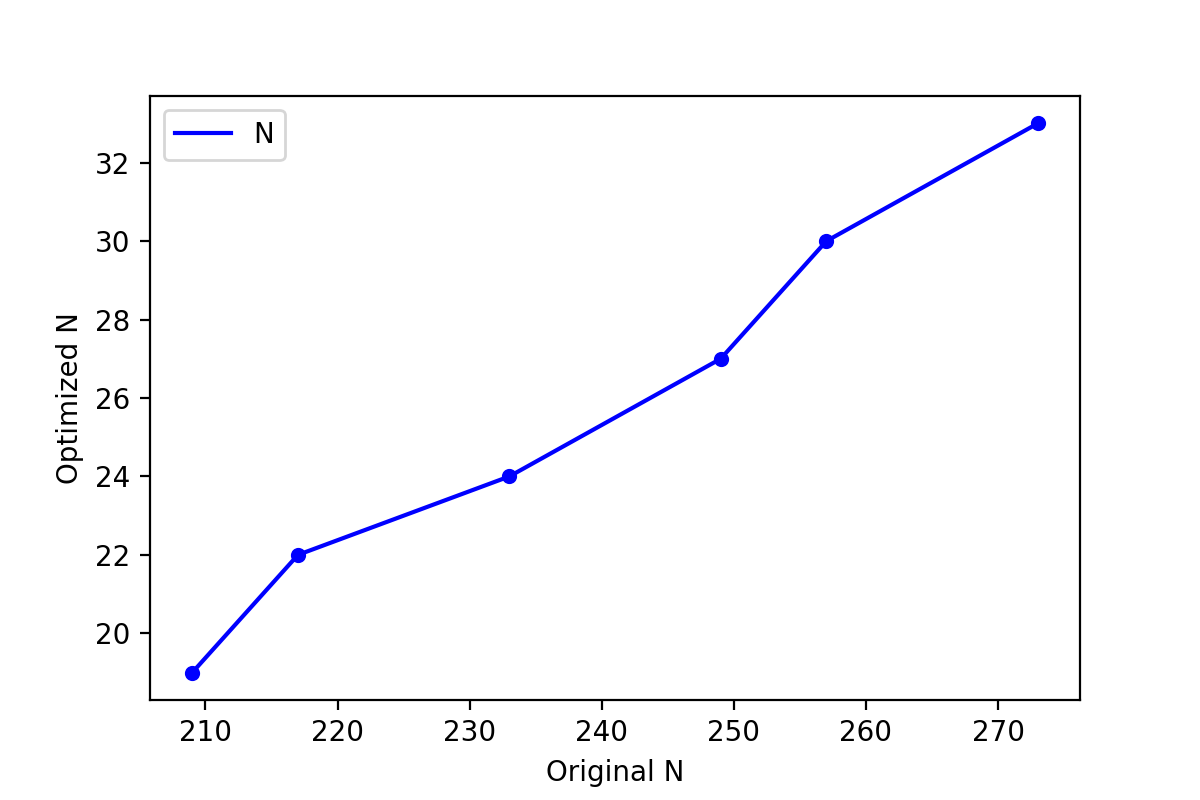
\includegraphics[width=0.8\linewidth]{figures/sudoku/s3_opt_row.png}
\caption{Riduzione delle righe della matrice A}\label{row:opt}
\end{figure}

\begin{figure}[h!]
\centering
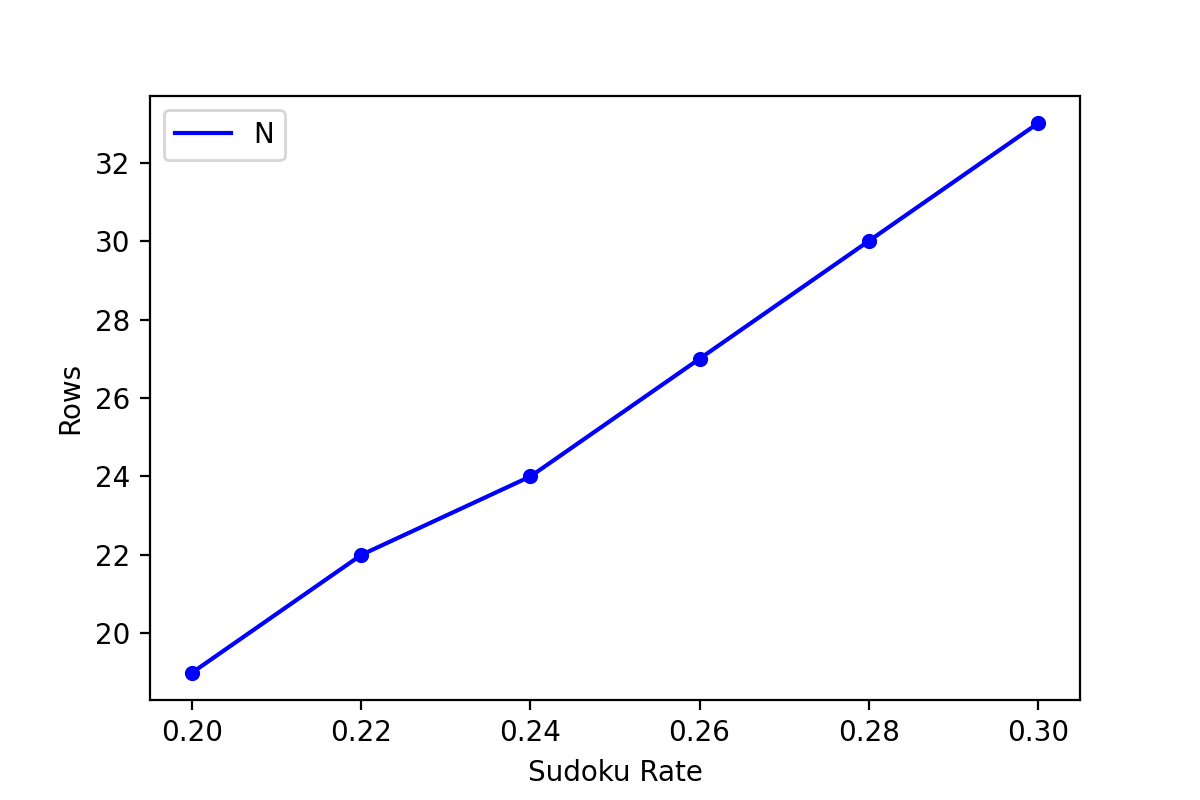
\includegraphics[width=0.8\linewidth]{figures/sudoku/s3_rate_row.png}
\caption{Rateo di riempimento del sudoku rispetto alle righe della matrice A}\label{rate:row}
\end{figure}

\subsection{Tempo di esecuzione}
Nella figura \ref{n:time} viene mostrata la performance temporale dell'algoritmo al variare delle righe della matrice A. Da questa si evince la crescita polinomiale del tempo di esecuzione. Si nota anche un grosso vantaggio della versione plus dell'algoritmo che aumenta all'aumentare di N.



\begin{figure}[h!]
\centering
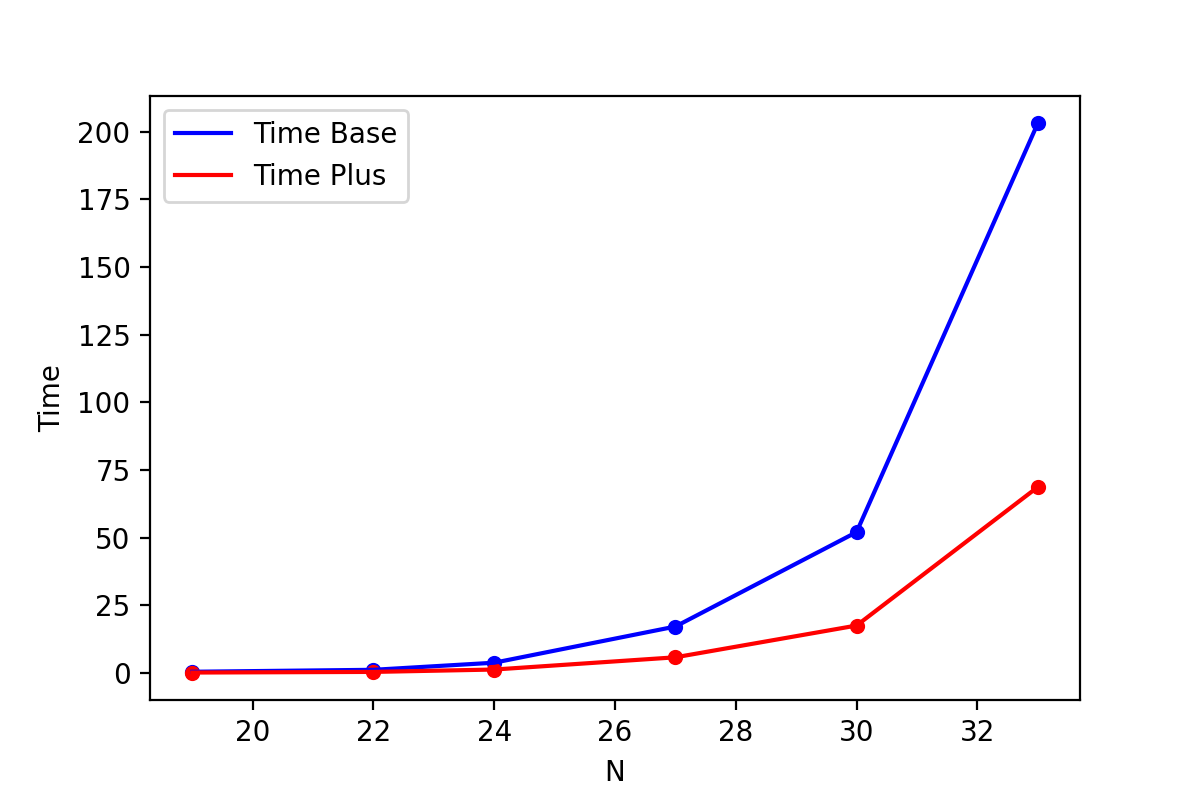
\includegraphics[width=0.8\linewidth]{figures/sudoku/s3_N_time.png}
\caption{Tempo al variare delle righe della matrice A}
\label{n:time}
\end{figure}

\subsection{Nodi visitati}
Nella figura \ref{row:nodes} viene mostrato il rapporto tra nodi totali dell'albero del problema confrontati con i nodi effettivamente visitati dall'algoritmo, rispetto all'aumentare di N. Essendo enormemente maggiori i primi, nella figura \ref{row:visited} vengono mostrati solamente i nodi visitati in modo da riuscire a coglierne l'andamento.


\begin{figure}[h!]
\centering
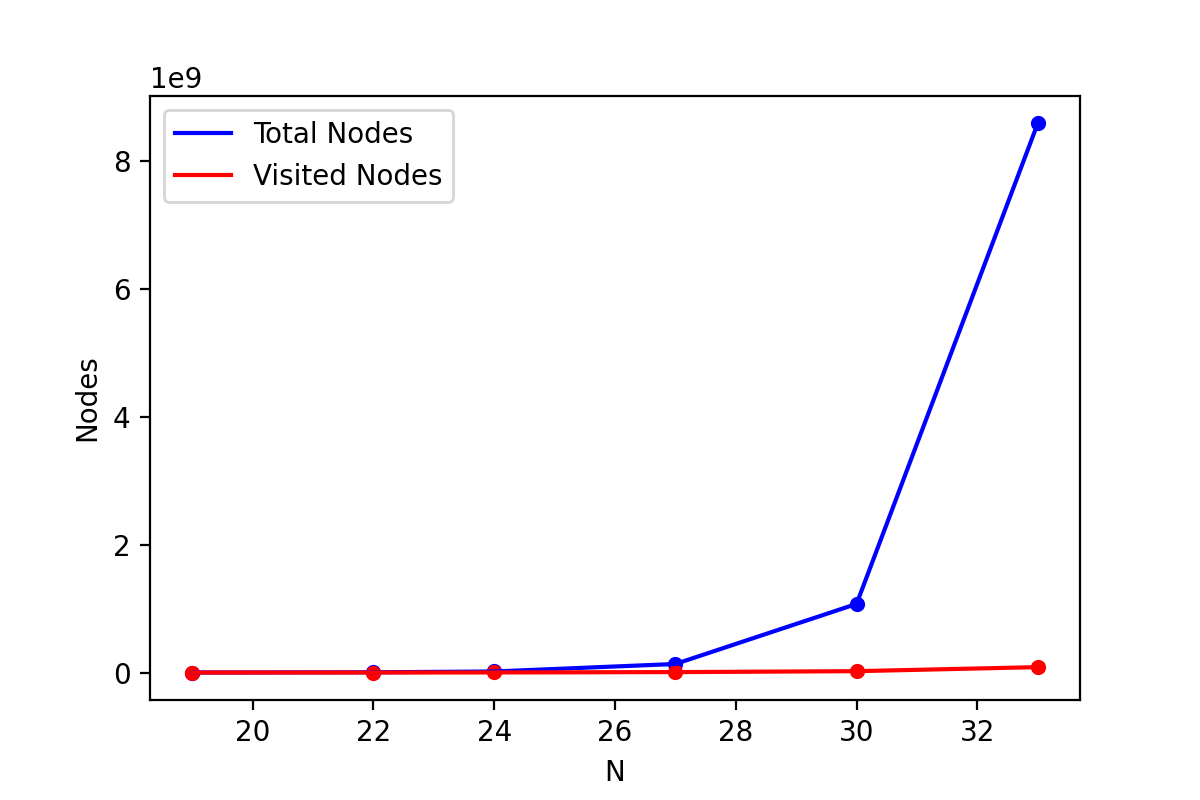
\includegraphics[width=0.8\linewidth]{figures/sudoku/s3_row_nodes.png}
\caption{Nodi totali e visitati al variare delle righe della matrice A}
\label{row:nodes}
\end{figure}


\begin{figure}[h!]
\centering
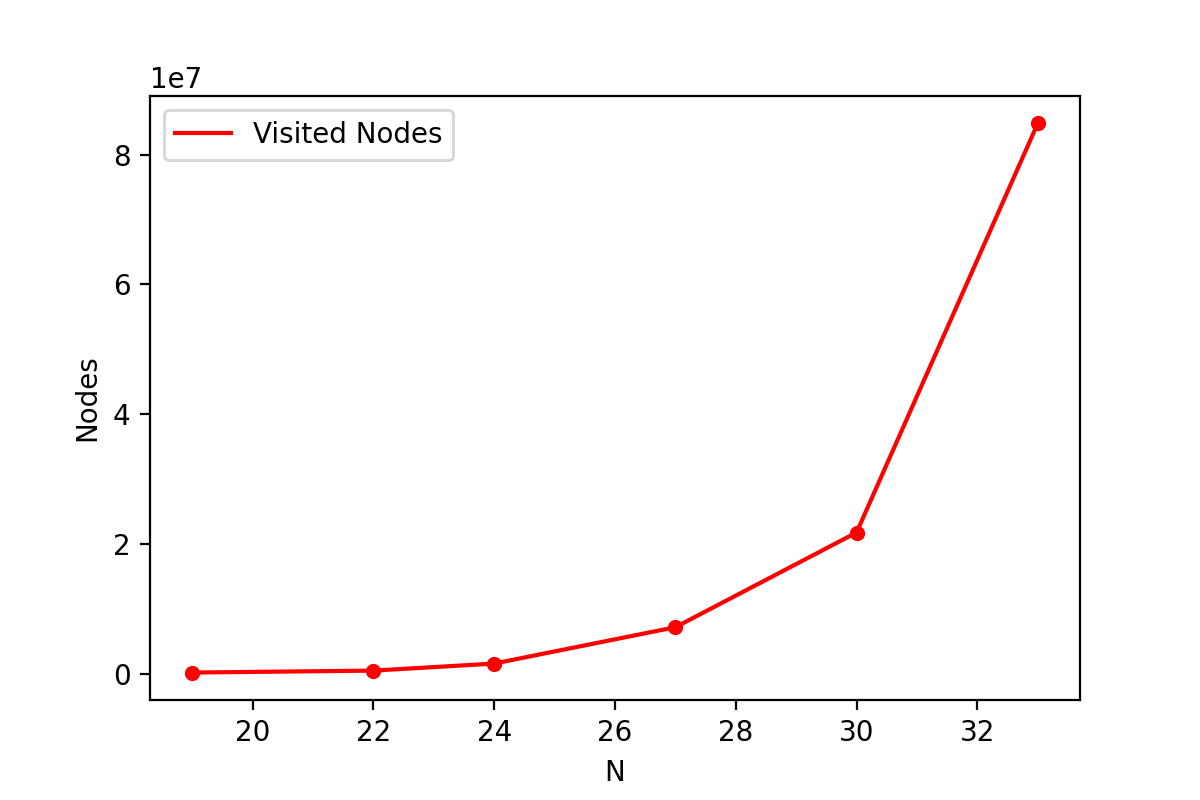
\includegraphics[width=0.8\linewidth]{figures/sudoku/s3_row_visited.png}
\caption{Nodi visitati al variare delle righe della matrice A}
\label{row:visited}
\end{figure}

\newpage{}

\subsection{Occupazione di memoria}
Nella figura \ref{row:mem} viene mostrata l'occupazione spaziale dell'algoritmo al variare della dimensione del problema in righe della matrice A, registrata profilando l'occupazione di memoria delle due funzioni che implementano lo stesso.

\begin{figure}[h!]
\centering
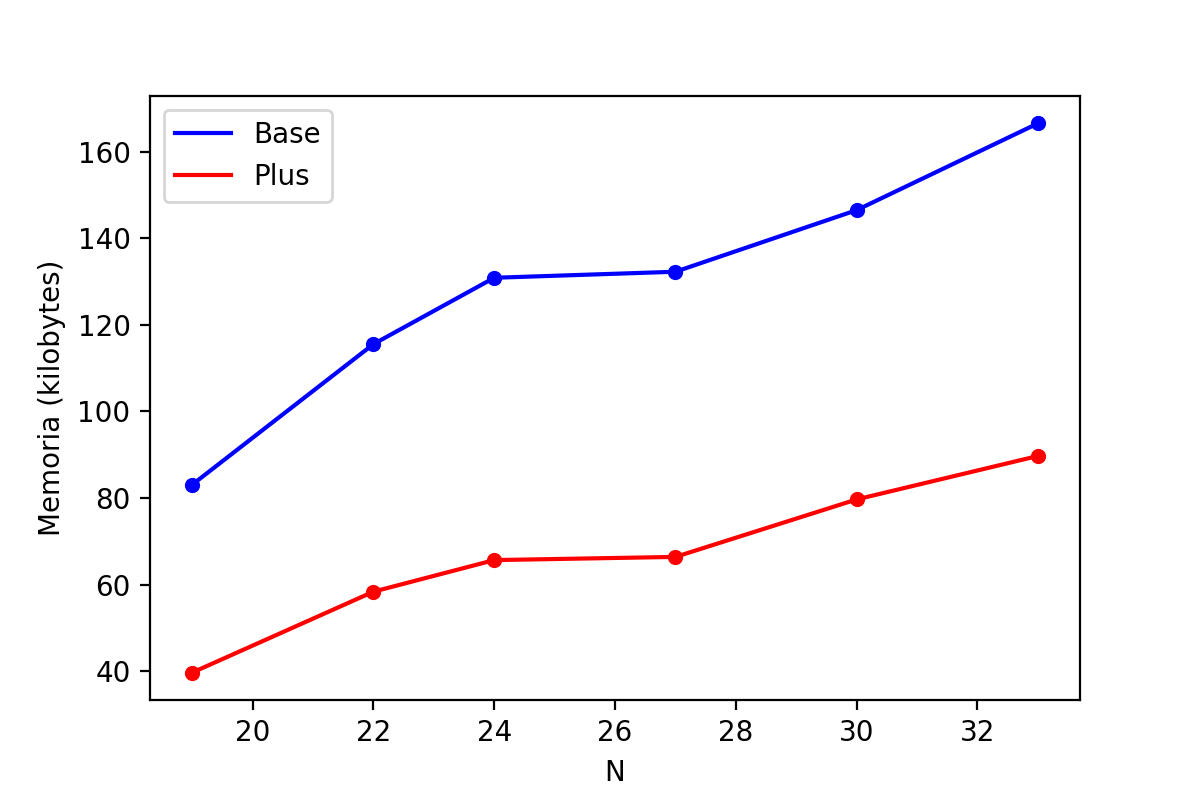
\includegraphics[width=0.8\linewidth]{figures/sudoku/s3_n_mem.png}
\caption{Occupazione spaziale dell'algoritmo al variare delle righe di A}
\label{row:mem}
\end{figure}


\newpage
\section{Random}

\subsection{Casi di test}
Siccome i casi di test creati per la risoluzione del sudoku mostrano l'andamento delle performance dell'algoritmo solo al variare delle righe, per completezza è stato testato l'algoritmo anche con matrici A create randomicamente in modo da mostrare la differenza di performance al variare delle colonne a parità di righe. Sono stati create 6 matrici A con 40 righe e colonne da 15 a 25 ed ognuna di esse è stata testata su 5 run facendo la media dei risultati. Come per il sudoku, la dimensione delle matrici è stata scelta dopo alcune prove empiriche come compromesso tra significatività dei risultati e fattibilità della computazione. È stata inoltre aggiunta una condizione opzionale che permette di assicurare sempre la presenza di almeno una soluzione nella matrice random creata, oltre a ciò non è stata eseguita alcuna ottimizzazione sull'input. Nella figura \ref{m:cov} viene mostrato il numero di soluzioni che diminuisce al crescere delle dimensioni del problema.

\begin{figure}[h!]
\centering
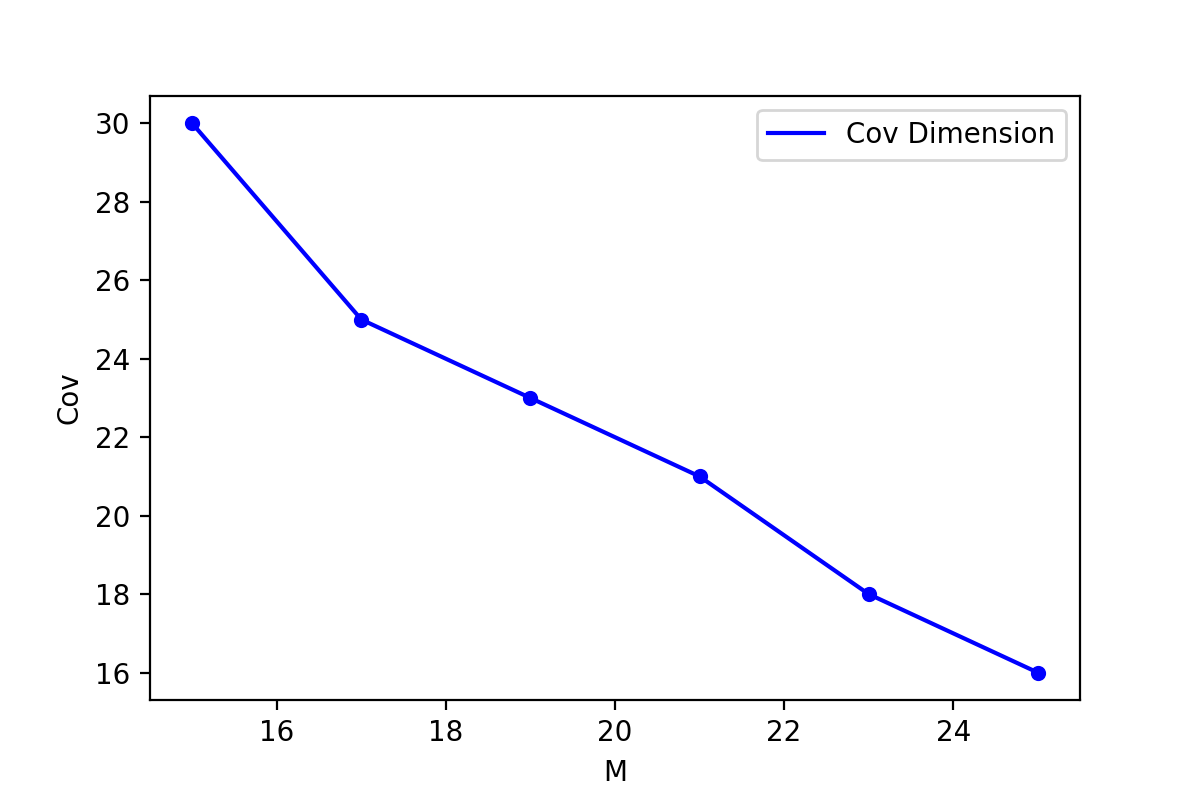
\includegraphics[width=0.9\linewidth]{figures/random/r_col_cov.png}
\caption{Numero di soluzioni al variare delle colonne della matrice A}
\label{m:cov}
\end{figure}


\subsection{Tempi di esecuzione}
Nella figura \ref{m:time} viene mostrata la performance temporale dell'algoritmo al variare delle colonne della matrice A. Da questa si evince la crescita polinomiale del tempo di esecuzione, come nel caso del sudoku. In questo caso la differenza di prestazioni tra le due vesioni dell'algoritmo è ridotta rispetto al sudoku ma si alza nel caso della versione che utilizza una stringa binaria per rappresentare la matrice.

\begin{figure}[h!]
\centering
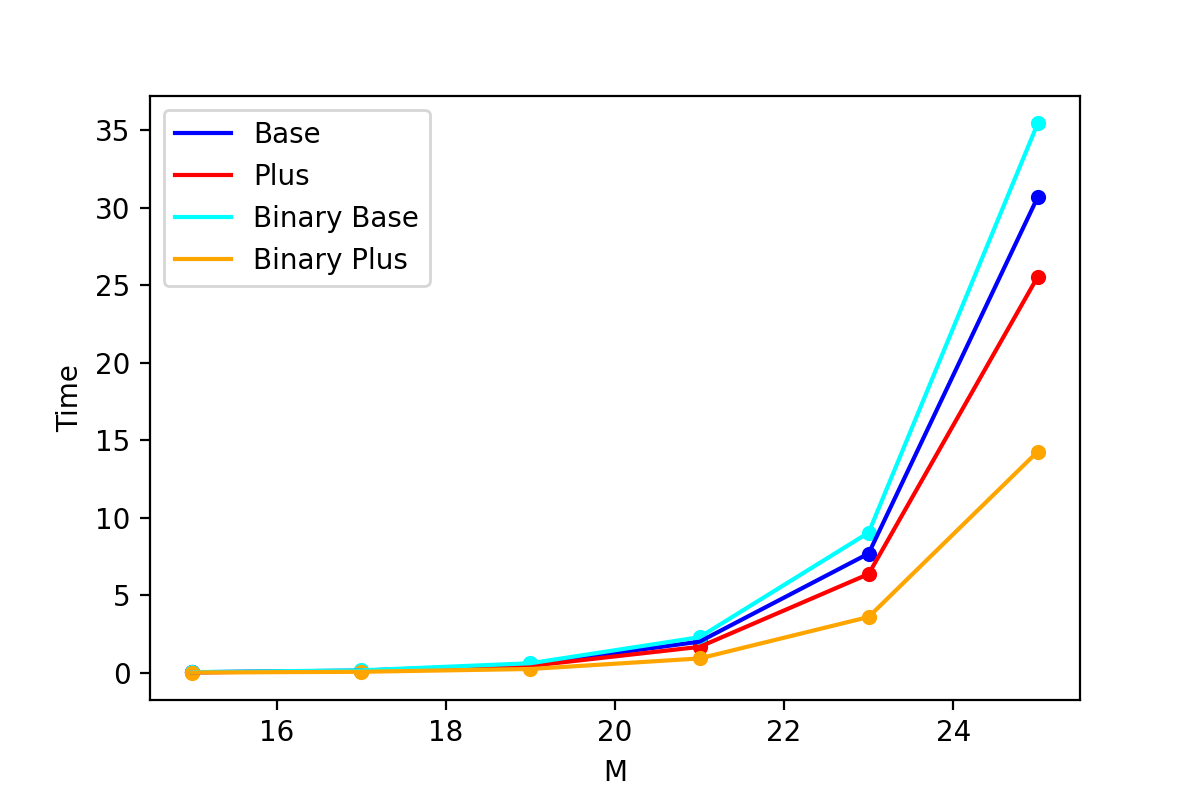
\includegraphics[width=0.8\linewidth]{figures/random/binary_time.png}
\caption{Tempo al variare delle colonne della matrice A}
\label{m:time}
\end{figure}

\newpage
\subsection{Nodi visitati}
Nella figura \ref{m:nodes} vengono mostrati i nodi dell'albero del problema visitati dall'algoritmo.

\begin{figure}[h!]
\centering
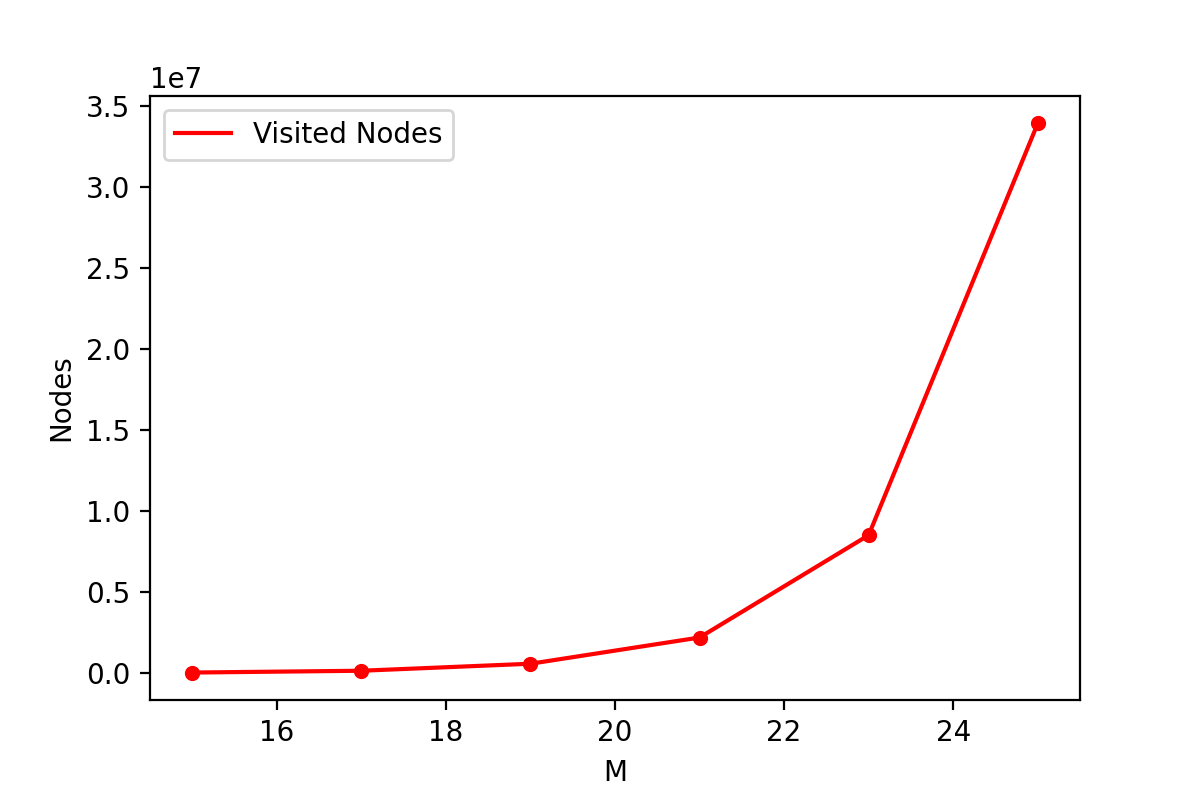
\includegraphics[width=0.8\linewidth]{figures/random/r_col_nodes.png}
\caption{Nodi visitati al variare delle colonne della matrice A}
\label{m:nodes}
\end{figure}

\newpage

\subsection{Occupazione di memoria}
Nella figura \ref{row:mem:r} viene mostrata l'occupazione spaziale dell'algoritmo al variare della dimensione del problema in colonne della matrice A, registrata profilando l'occupazione di memoria delle due funzioni che implementano lo stesso.

\begin{figure}[h!]
\centering
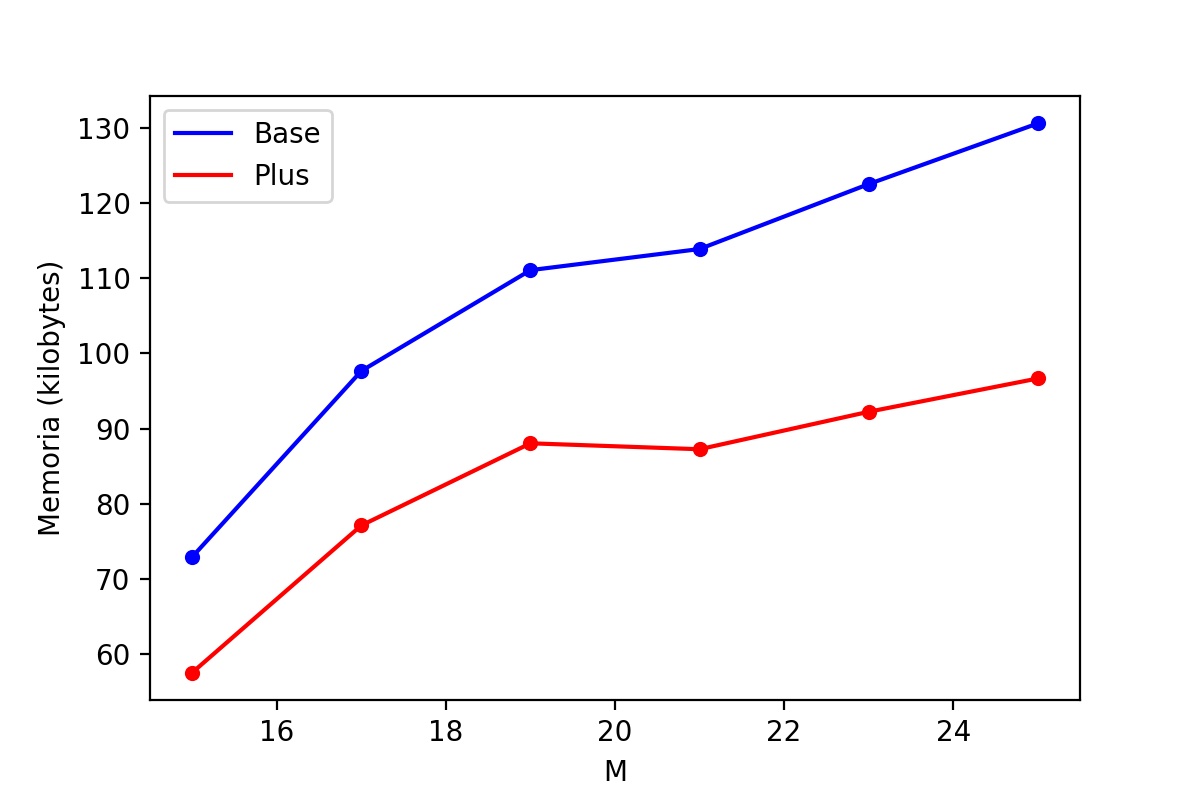
\includegraphics[width=0.8\linewidth]{figures/random/r_m_mem.png}
\caption{Occupazione spaziale dell'algoritmo al variare delle colonne di A}
\label{row:mem:r}
\end{figure}

\chapter{Conclusioni e lavori futuri}
\section{Conclusioni e osservazioni}
I risultati ottenuti mostrano che l’algoritmo sia poco efficiente in termini di performance temporali al crescere della dimensione del problema: esistono infatti altri algoritmi atti a risolvere lo stesso problema molto più efficienti, come l’algoritmo di Knuth che adopera i Dancing Links.

Confrontando gli algoritmi base e plus quest’ultimo è risultato più veloce in tutti i test, andando inoltre ad ampliare il distacco dal base nel caso dell’implementazione della rappresentazione binaria dell’input.

Avendo scelto un linguaggio di programmazione ad alto livello come Python per la sua flessibilità e facilità di prototipazione e riuso del codice, nonchè per nostra maggiore familiarità con il linguaggio, è possibile che esso contribuisca alle non ottimali performance del programma.

\section{Lavori futuri}
Riteniamo che all’algoritmo in se non si possano effettuare variazioni che vadano ad influire particolarmente sulla velocità di esecuzione (fermo restando di utilizzare esattamente questo algoritmo senza variarne il funzionamento basilare).

Si potrebbero svolgere nuovi test sia con una versione più aggiornata di Python, in particolare la 3.11, ultima uscita, che ha aumentato le performance generali del linguaggio, oppure con un diverso linguaggio di programmazione a più basso livello come C.


\appendix
\chapter{Usage Report}

Per utilizzare il codice prodotto, clonare la repository e seguire le istruzioni presenti nel readme per la generazione degli input, infine eseguire ExactCover.


Repository del progetto: [\url{https://github.com/H3isenb3rg/ExactCover2022}]

\label{a:urep}
Il progetto è stato sviluppato utilizzando i seguenti strumenti/linguaggi/librerie:\\
Python [\url{https://www.python.org/}]\\
Numpy [\url{https://numpy.org/}]\\
Filprofiler [\url{https://github.com/pythonspeed/filprofiler}]\\
Pyplot [\url{https://matplotlib.org/stable/index.html}]





\vspace*{\fill}
\subsection*{CopyRight}
\begin{center}
\footnotesize
\begin{tabular}{p{0.25\textwidth} p{0.7\textwidth}}
\raisebox{-12mm}{
\includegraphics[width=4cm]{figures/by-nc-sa.png}}   &  This work is licensed by the authors under the license Creative Commons 4.0 CC Attribution-NonCommercial-ShareAlike (\url{https://creativecommons.org/licenses/by-nc-sa/4.0/legalcode}). \\ 
 & You can reuse and share the material also for derivative work within the limits allowed by the license and with the proper attribution. 
 \end{tabular}
\end{center}

\end{document}